
\section{Data Analysis}
\label{sec:data-analysis}

The TIM Hamiltonian for calculating the occupation number versus Trotter step served as a quantum computing application example for studying the stability and reproducibility of these computations on the Boeblingen platform.  

In this section we will focus on analyzing the results from a direct calculation of the TIM occupation index and from a detailed study of 2 different sets of CNOT gate configurations (circuit 1 and circuit 2) 
using cycle benchmarking based on the gate sequences in the TIM Hamiltonian. 





show this issue 



Measurements were done with the occupation index and for cycle benchmakring of circuits 1 and 2 at specific time periods within the same day, at the same set of specific time periods for different days, and also with the placement of these two circuits on groups of 4 qubits located in different physically distinct areas on the Boeblingen platform. These results are analyzed and summarized for inter-day (Sect.~\ref{inter-day-analysis}) and intra-day (Sect.~\ref{intra-day-analysis}) calibration drift of the qubits and on concurrent computation inconsistencies (Sect.~\ref{sec:concurrent-computation-inconsistency-analysis}) running the TIM circuit using different qubits within the Boeblingen platform.  In addition to these studies, the cycle benchmarking computations are compared to the randomized benchmarking IBM calibration measurements for the relevant 2-qubit gates that measure how accurately these computations reflect sources of hardware errors on the Boeblingen chip.

\subsection{Inter-day Calibration Drift}
\label{inter-day-analysis}


We observed inter-day calibration drift throughout the time period when measurements were done on Boeblingen.  These included the occupation index versus Trotter step for the TIM Hamiltonian and the application of circuits 1 and 2 to different qubit layouts at the same time each day on different days. 

An example illustrating this inter-day calibration drift can be seen with both the TIM and cycle benchmarking using circuit 1 applied to the qubits on layout2 for runs done on the morning of January 24, 2021 and January 29, 2021.  

Figure \ref{fig:n1_Story4} shows the occupation index 1 calculated as a function of time from the morning runs of layout 2 (qubits [6, 7, 12, 11]) on days 01/24/2021 and 01/29/2021 compared to exact Trotter approximation.  

Cycle benchmarking was applied using circuit 1 on layout 2 for both the morning of January 24, 2021 and January 29, 2021.  Following the procedure for cycle benchmarking outlined in Appendix \ref{sec:cyclebenchmarking} measurements of the decaying exponential curves of the expectation values versus randomized Clifford gate sequences of length 2, 10 and 22 were recorded for all 16 combinations of identity and z gates for the 4 qubits.  A curve fitting routine was applied to the 3 sets of decay curves to calculate the individual process infidelity for each of the 16 combinations of Pauli I and Z gate decay terms as shown in Figure \ref{fig:PauliInfidelities27_29_Story4}.  The figure shows the comparison of the results from the calculations of the Pauli infidelities for each hard cycle with the solid line and the shaded region showing the overall combined process infidelity and the error bars from these calculations. 

The team retrieved the measured values for the layout 2 single qubit error measurements ( Table~\ref{table:Layout2-single-qubit-error-morning-1-24-and-1-29} ) and the layout 2 two qubit error measurements ( Table~\ref{table:Two-qubit-gate-error-layout2-on-1-24-and-1-29} ) from the 
recorded data of IBM full calibration of Boeblingen's backend properties that were done on the morning of January 24th and January 29th at 4 am.   Using equation \eqref{eq:err_rate}
% eq.(\ref{eq:avg process to gate infidelity conversion}) 
the average gate infidelity measurements recorded in the IBM backend properties for qubits 6, 7, 11, and 12 on both teh 24th and 29th were converted to average process infidelity quantities.  Both the cycle benchmarking calculations and process infidelty from the IBM backend gate error measurements that were converted to process infidelities were then plotted together in Figure \ref{fig:processinfidelitiesStory4}.   

Finally the QCAP bound as a function of number Trotter steps calculated using randomized benchmarking (QCAP$_{\text{RB}}$) (right axis) and cycle benchmarking (QCAP$_{\text{CB}}$) (left axis) from the morning runs of circuit1 on layout 2 (qubits [6, 7, 12, 11]) on 01/24/2021 and 01/29/2021 were plotted in  Fig.~\ref{fig:QCAPCB_RB_Story4}.


  












\textbf{This table needs to be completed}

\begin{table*}[ht!]
\begin{tabular}{|c|c|c|c|c|c|c|}
\hline
\multicolumn{7}{|c|}{\textbf{Layout 2 Single Qubit Error}}                                                                                                                                                                                                                                                                                                    \\ \hline
\textbf{}                                                                          & \textbf{Qubits}            & \textbf{\begin{tabular}[c]{@{}c@{}}$T_1$\\ ( $\mu$s)\end{tabular}} & \textbf{\begin{tabular}[c]{@{}c@{}}$T_2$\\ ( $\mu$s)\end{tabular}} & \textbf{Readout Error}         & \textbf{U1}              & \textbf{U2}                       \\ \hline
                                                                                   & \cellcolor[HTML]{FFFFFF}6  & \cellcolor[HTML]{FFFFFF}67.1                                         & \cellcolor[HTML]{FFFFFF}99.9                                         & \cellcolor[HTML]{FFFFFF}0.0254 & \cellcolor[HTML]{DAE8FC} & \cellcolor[HTML]{DAE8FC}          \\ \cline{2-7} 
                                                                                   & \cellcolor[HTML]{FFFFFF}7  & \cellcolor[HTML]{FFFFFF}94.8                                         & \cellcolor[HTML]{FFFFFF}86.8                                         & \cellcolor[HTML]{FFFFFF}0.023  & \cellcolor[HTML]{DAE8FC} & \cellcolor[HTML]{DAE8FC}          \\ \cline{2-7} 
                                                                                   & \cellcolor[HTML]{FFFFFF}12 & \cellcolor[HTML]{FFFFFF}97.5                                         & \cellcolor[HTML]{FFFFFF}88.5                                         & \cellcolor[HTML]{FFFFFF}0.0313 & \cellcolor[HTML]{DAE8FC} & \cellcolor[HTML]{DAE8FC}          \\ \cline{2-7} 
\multirow{-4}{*}{\begin{tabular}[c]{@{}c@{}}01/24/2021\\ Morning Run\end{tabular}} & \cellcolor[HTML]{FFFFFF}11 & \cellcolor[HTML]{FFFFFF}95.1                                         & \cellcolor[HTML]{FFFFFF}71.6                                         & \cellcolor[HTML]{FFFFFF}0.0355 & \cellcolor[HTML]{DAE8FC} & \cellcolor[HTML]{DAE8FC}\textit{} \\ \hline
                                                                                   & \cellcolor[HTML]{FFFFFF}6  & \cellcolor[HTML]{FFFFFF}24.1                                         & \cellcolor[HTML]{FFFFFF}4.97                                         & \cellcolor[HTML]{FFFFFF}0.0919 & \cellcolor[HTML]{DAE8FC} & \cellcolor[HTML]{DAE8FC}          \\ \cline{2-7} 
                                                                                   & \cellcolor[HTML]{FFFFFF}7  & \cellcolor[HTML]{FFFFFF}78.8                                         & \cellcolor[HTML]{FFFFFF}103.4                                        & \cellcolor[HTML]{FFFFFF}0.0284 & \cellcolor[HTML]{DAE8FC} & \cellcolor[HTML]{DAE8FC}          \\ \cline{2-7} 
                                                                                   & \cellcolor[HTML]{FFFFFF}12 & \cellcolor[HTML]{FFFFFF}80.8                                         & \cellcolor[HTML]{FFFFFF}114.6                                        & \cellcolor[HTML]{FFFFFF}0.0347 & \cellcolor[HTML]{DAE8FC} & \cellcolor[HTML]{DAE8FC}          \\ \cline{2-7} 
\multirow{-4}{*}{\begin{tabular}[c]{@{}c@{}}01/29/2021\\ Morning Run\end{tabular}} & \cellcolor[HTML]{FFFFFF}11 & \cellcolor[HTML]{FFFFFF}48.4                                         & \cellcolor[HTML]{FFFFFF}87.8                                         & \cellcolor[HTML]{FFFFFF}0.0322 & \cellcolor[HTML]{DAE8FC} & \cellcolor[HTML]{DAE8FC}          \\ \hline
\end{tabular}
\label{table:Layout2-single-qubit-error-morning-1-24-and-1-29}
\caption{Values for single qubit errors for qubits [6, 7, 11, 12] extracted from the recorded IBM back-end properties immediately after IBM completed a full re-calibration of the Boeblingen quantum chip on the morning of January 24, 2021 and January 29, 2021}
\end{table*}


The comparison of the computed values of the error rates for the Layout 2, two-qubit pairs 





\begin{table}[ht!]
\begin{tabular}{|c|c|c|}
\hline
\multicolumn{3}{|c|}{\textbf{Layout 2 Two-Qubit Gate Error}}                                                                            \\ \hline
\textbf{}                                                                          & \textbf{Qubits}               & \textbf{CNOT Error} \\ \hline
                                                                                   & \cellcolor[HTML]{FFFFFF}[6,7] & 0.00726             \\ \cline{2-3} 
                                                                                   & [7,12]                        & 0.00903             \\ \cline{2-3} 
\multirow{-3}{*}{\begin{tabular}[c]{@{}c@{}}01/24/2021\\ Morning Run\end{tabular}} & [12,11]                       & 0.00808             \\ \hline
                                                                                   & \cellcolor[HTML]{FFFFFF}[6,7] & 0.026               \\ \cline{2-3} 
                                                                                   & [7,12]                        & 0.0100              \\ \cline{2-3} 
\multirow{-3}{*}{\begin{tabular}[c]{@{}c@{}}01/29/2021\\ Morning Run\end{tabular}} & [12,11]                       & 0.00899             \\ \hline
\end{tabular}
\label{table:Two-qubit-gate-error-layout2-on-1-24-and-1-29} 
\caption{Values for two qubit error pairs [6, 7], [7,12], [12, 11] extracted from the recorded IBM back-end properties immediately after IBM completed a full re-calibration of the Boeblingen quantum chip on the morning of January 24, 2021 and January 29, 2021 \textbf{mention error bars in text} and the error values for the two qubit pairs from cycle 2, 3, and 4 from the cycle benchmarking computations.}
\end{table}


\begin{figure}[H]
    % \centering
    % \includegraphics[width=2.2\columnwidth]{final_plot.pdf}
    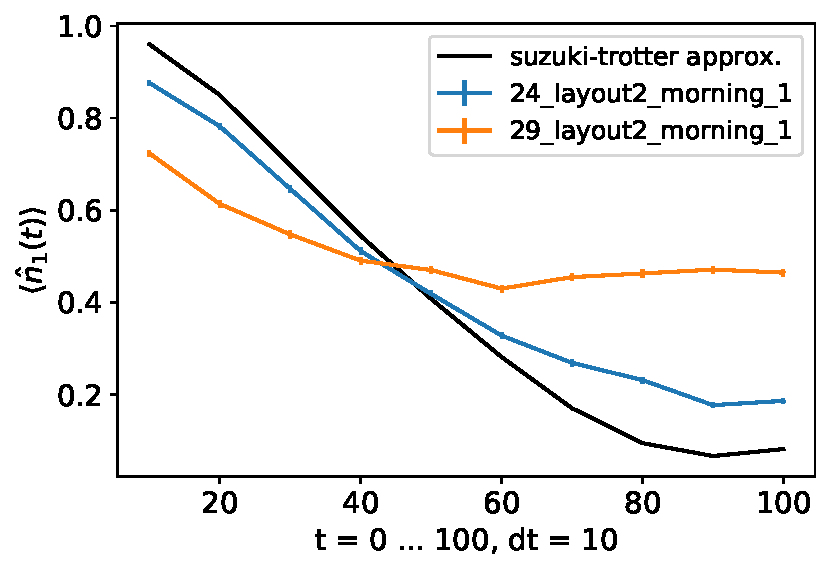
\includegraphics[scale=0.5]{TIM_[24, 29]_[layout2]_[morning]_n1.pdf}
    \caption{The particle number in site 1 calculated as a function of time from morning run of layout 2 (qubits [6, 7, 12, 11]) on days 01/24/2021 and 01/29/2021 compared to exact Suzuki-Trotter approximation.}
    \label{fig:n1_Story4}
\end{figure}




\begin{figure*}[ht!]
    % \centering
    % \includegraphics[width=2.2\columnwidth]{final_plot.pdf}
    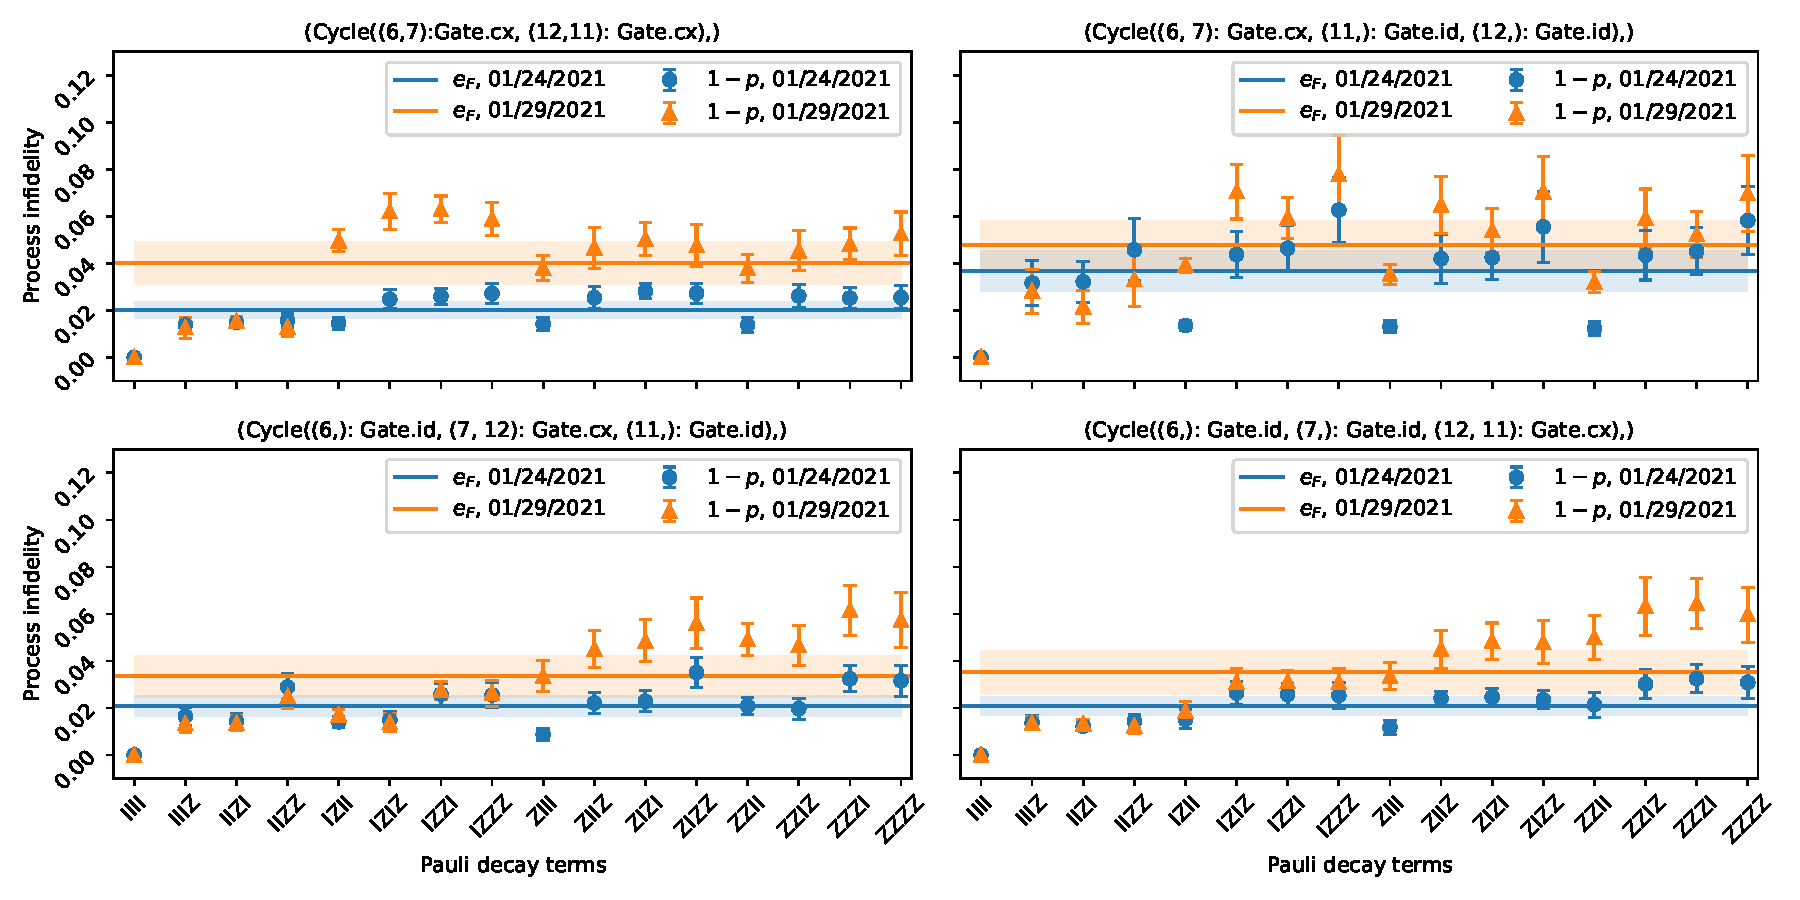
\includegraphics[scale=0.56]{CBPauliInfidelities_24_29_01_2021_MorningRun_Layout2_Cycle1_2_3_4.pdf}
    \caption{The Pauli infidelities for each hard cycle calculated for each Pauli decay term from morning run of layout 2 (qubits [6, 7, 12, 11]) on days 01/24/2021 and 01/29/2021. The shaded regions show the error on the process infidelity and the error bars on the markers show the statistical errors on Pauli decay terms. }
    \label{fig:PauliInfidelities27_29_Story4}
\end{figure*}



\begin{figure}[H]
    % \centering
    % \includegraphics[width=2.2\columnwidth]{final_plot.pdf}
    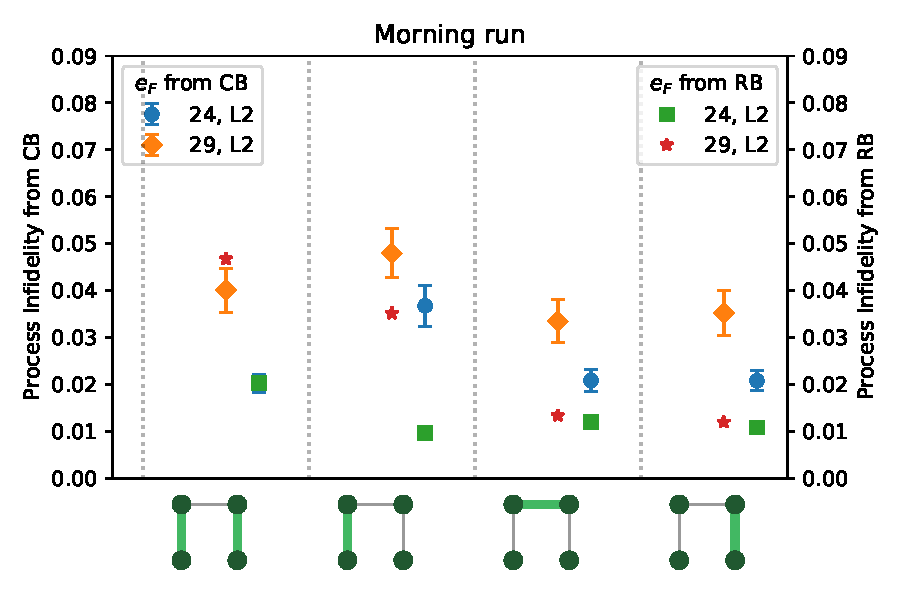
\includegraphics[scale=0.5]{ProcessInfidelities_CB_RB_Data_01_24_2021_01_292021_Layout2aligned.pdf}
    \caption{The process infidelities calculated using randomized benchmarking (RB) (right axis) and cycle benchmarking (CB) (left axis) from the morning runs of circuit 1 on layout 2 (qubits [6, 7, 12, 11]) on 01/24/2021 and 01/29/2021.  the two qubit CNOT cycles 1, 2, 3, and 4 are identified along the horizontal axis from left to right}
    \label{fig:processinfidelitiesStory4}
\end{figure}
  

\begin{figure}[H]
    % \centering
    % \includegraphics[width=2.2\columnwidth]{final_plot.pdf}
    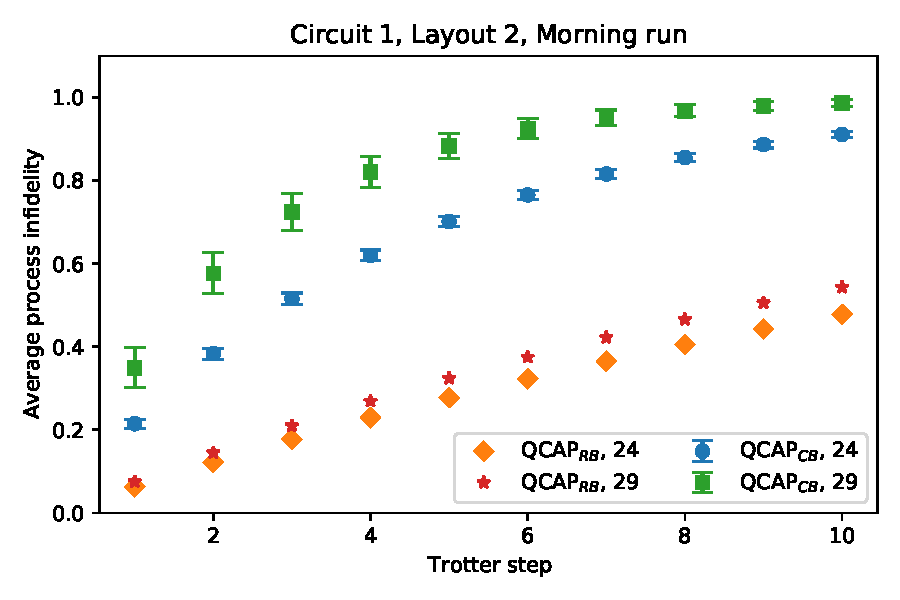
\includegraphics[scale=0.56]{QCAP_CB_RB_Data_01_24_29_2021_Layout_2C1.pdf}
    \caption{The QCAP bound as a function of number Trotter steps calculated using randomized benchmarking (QCAP$_{\text{RB}}$) (right axis) and cycle benchmarking (QCAP$_{\text{CB}}$) (left axis) from morning run of layout 2 (qubits [6, 7, 12, 11]) on days 01/24/2021 and 01/29/2021. The plotted error bars only show the statistical error.}
    \label{fig:QCAPCB_RB_Story4}
\end{figure}



% Figure \ref{fig:4-CBRawData_24_01_2021_MorningRun_Layout2}
%for the 24th.  Figure \ref{fig:4-CBRawData_29_01_2021_MorningRun_Layout2} for the 29th

%\begin{figure*}[ht!]
    % \centering
    % \includegraphics[width=2.2\columnwidth]{final_plot.pdf}
%    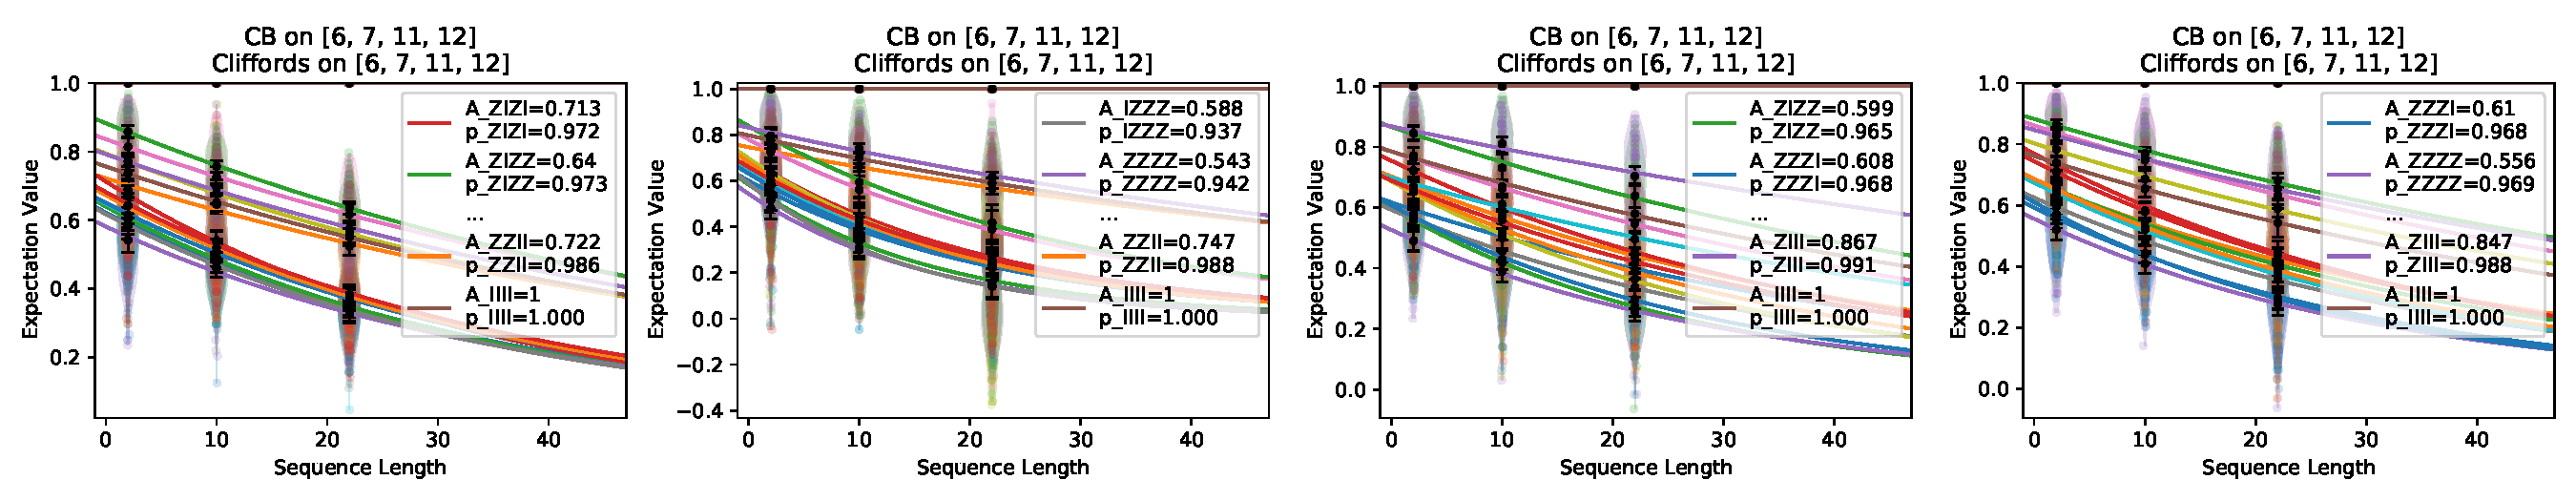
\includegraphics[scale=0.4]{4-CBRawData_24_01_2021_MorningRun_Layout2.pdf}
%    \caption{Expectation values of the Pauli group versus sequence length plotted for random Pauli gate sequences of length 2, 10 and 22 showing decay curves for all I and Z gate combinations with both amplitude (A) and slope (p) from morning run of layout 2 (qubits [6, 7, 12, 11]) on 01/24/2021.}
%    \label{fig:4-CBRawData_24_01_2021_MorningRun_Layout2}
%\end{figure*}

%\begin{figure*}[ht!]
    % \centering
    % \includegraphics[width=2.2\columnwidth]{final_plot.pdf}
%    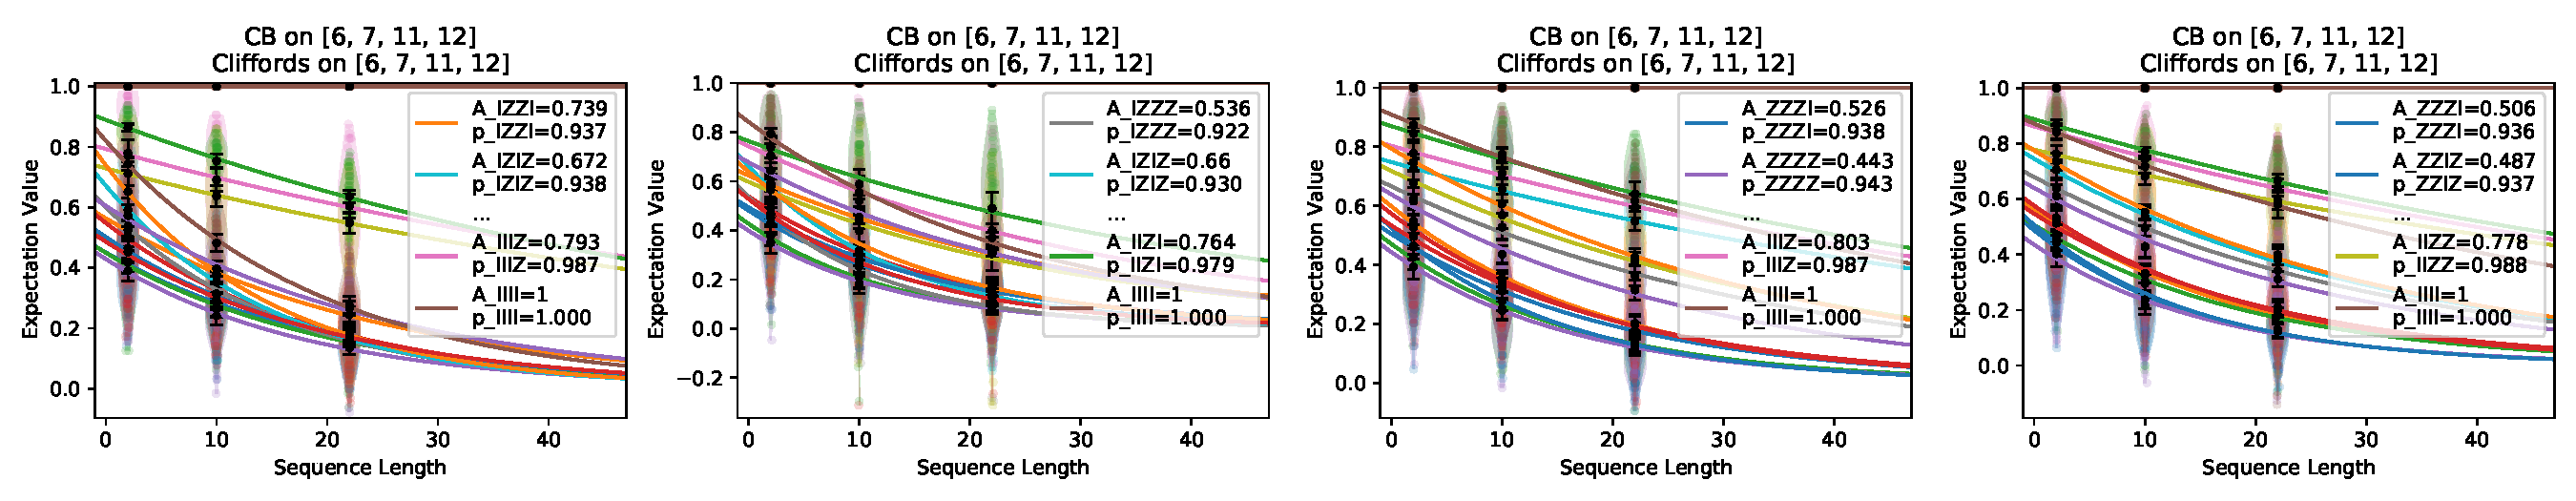
\includegraphics[scale=0.4]{4-CBRawData_29_01_2021_MorningRun_Layout2.pdf}
%    \caption{Expectation values of the Pauli group versus sequence length plotted for random Pauli gate sequences of length 2, 10 and 22 showing decay curves for all I and Z gate combinations with both amplitude (A) and slope (p) from morning run of layout 2 (qubits [6, 7, 12, 11]) on 01/29/2021.}
%    \label{fig:4-CBRawData_29_01_2021_MorningRun_Layout2}
%\end{figure*}

















\subsection{Intra-day Calibration Drift}
\label{intra-day-analysis}


We also observed calibration drift throughout different time periods within the same day when measurements were done on Boeblingen.  
These included the occupation index versus Trotter step for the TIM Hamiltonian and the application of circuits 1 and 2 to different qubit layouts at the same time each day on different days. 

Examples illustrating this intra-day calibration drift can be seen with both the TIM and cycle benchmarking data using circuit 1 applied to the qubits on layout2 for runs done on January 27, 2021 and January 30, 2021.  



From the January 27th data the detailed variances between the morning and night 2 qubit re-calibrations of qubits 6, 7, 11, and 12 can be seen when comparing the Pauli infidelities for each hard cycle calculated for each Pauli decay term from morning run of layout 2 (qubits [6, 7, 12, 11]) on 01/27/2021 
Fig.~\ref{fig:PauliInfidelities27Morning_Story6}, 
the night run shown in Fig.~\ref{fig:PauliInfidelities27Night_Story6} 
and the overall process infidelity for cycles 1, 2, 3, and 4 in Fig.~\ref{fig:processinfidelitiesStory6} for January 27th.

\begin{figure*}[ht!]
    % \centering
    % \includegraphics[width=2.2\columnwidth]{final_plot.pdf}
    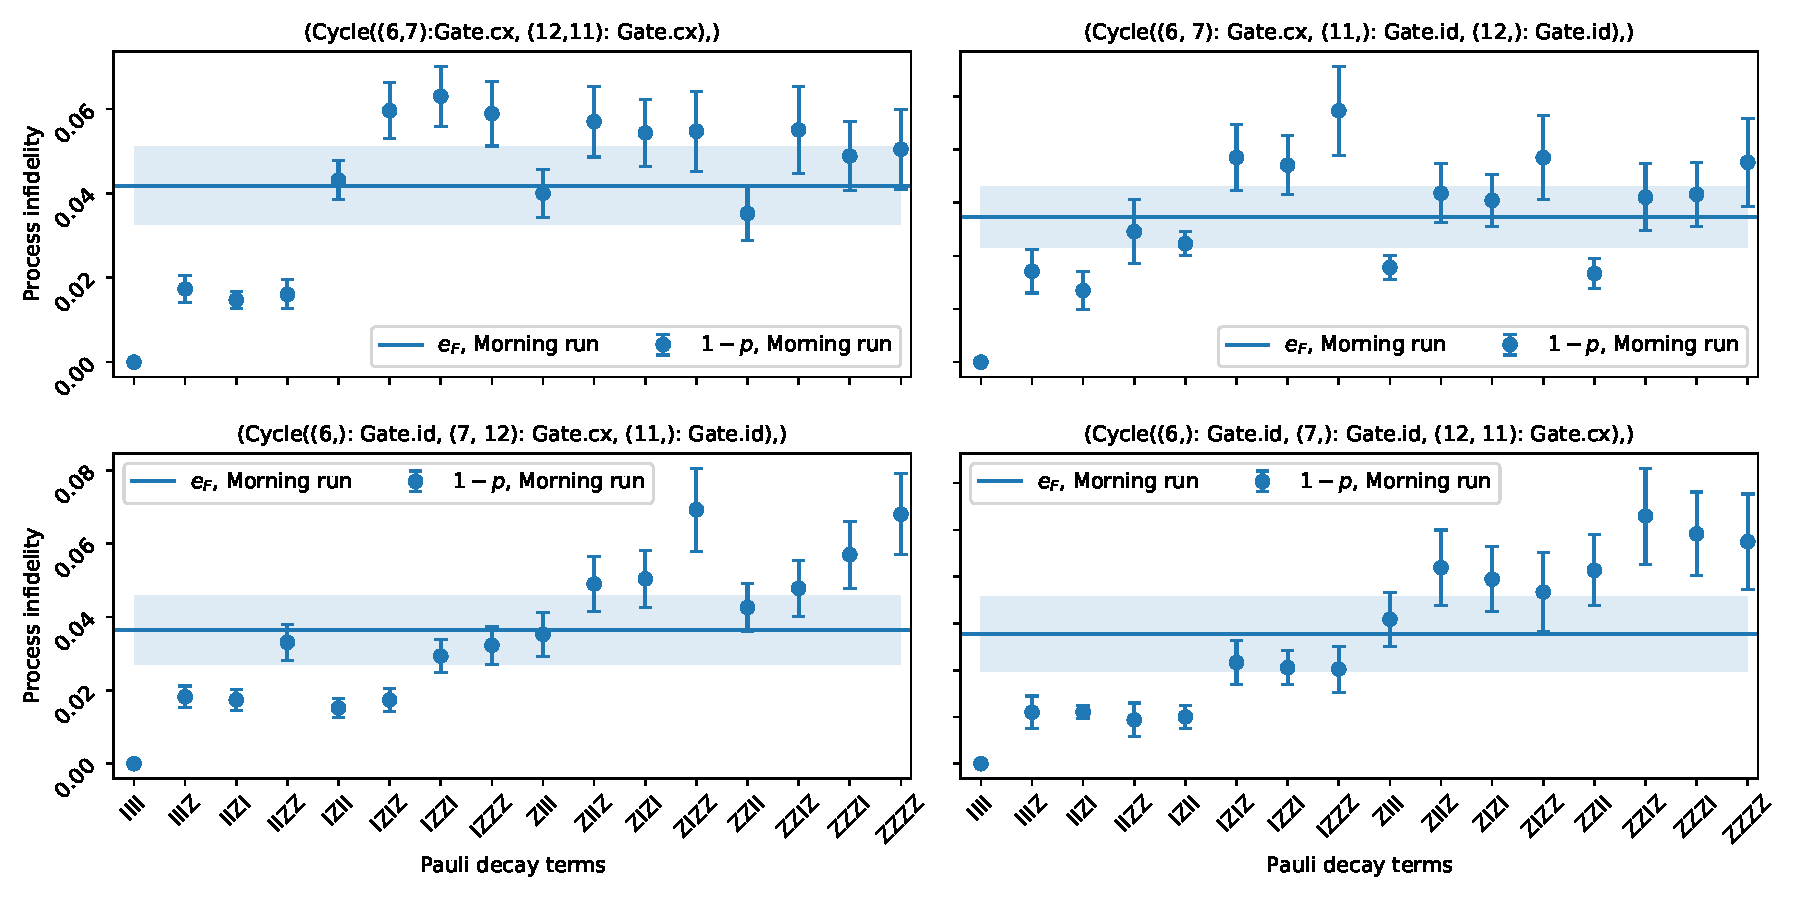
\includegraphics[scale=0.56]{CBPauliInfidelities_27_01_2021_MorningRun_Layout2_Cycle1_2_3_4.pdf}
    \caption{The Pauli infidelities for each hard cycle calculated for each Pauli decay term from morning run of layout 2 (qubits [6, 7, 12, 11]) on day 01/27/2021. The shaded regions show the error on the process infidelity and the error bars on the markers show the statistical errors on Pauli decay terms. }
    \label{fig:PauliInfidelities27Morning_Story6}
\end{figure*}


\begin{figure*}[ht!]
    % \centering
    % \includegraphics[width=2.2\columnwidth]{final_plot.pdf}
    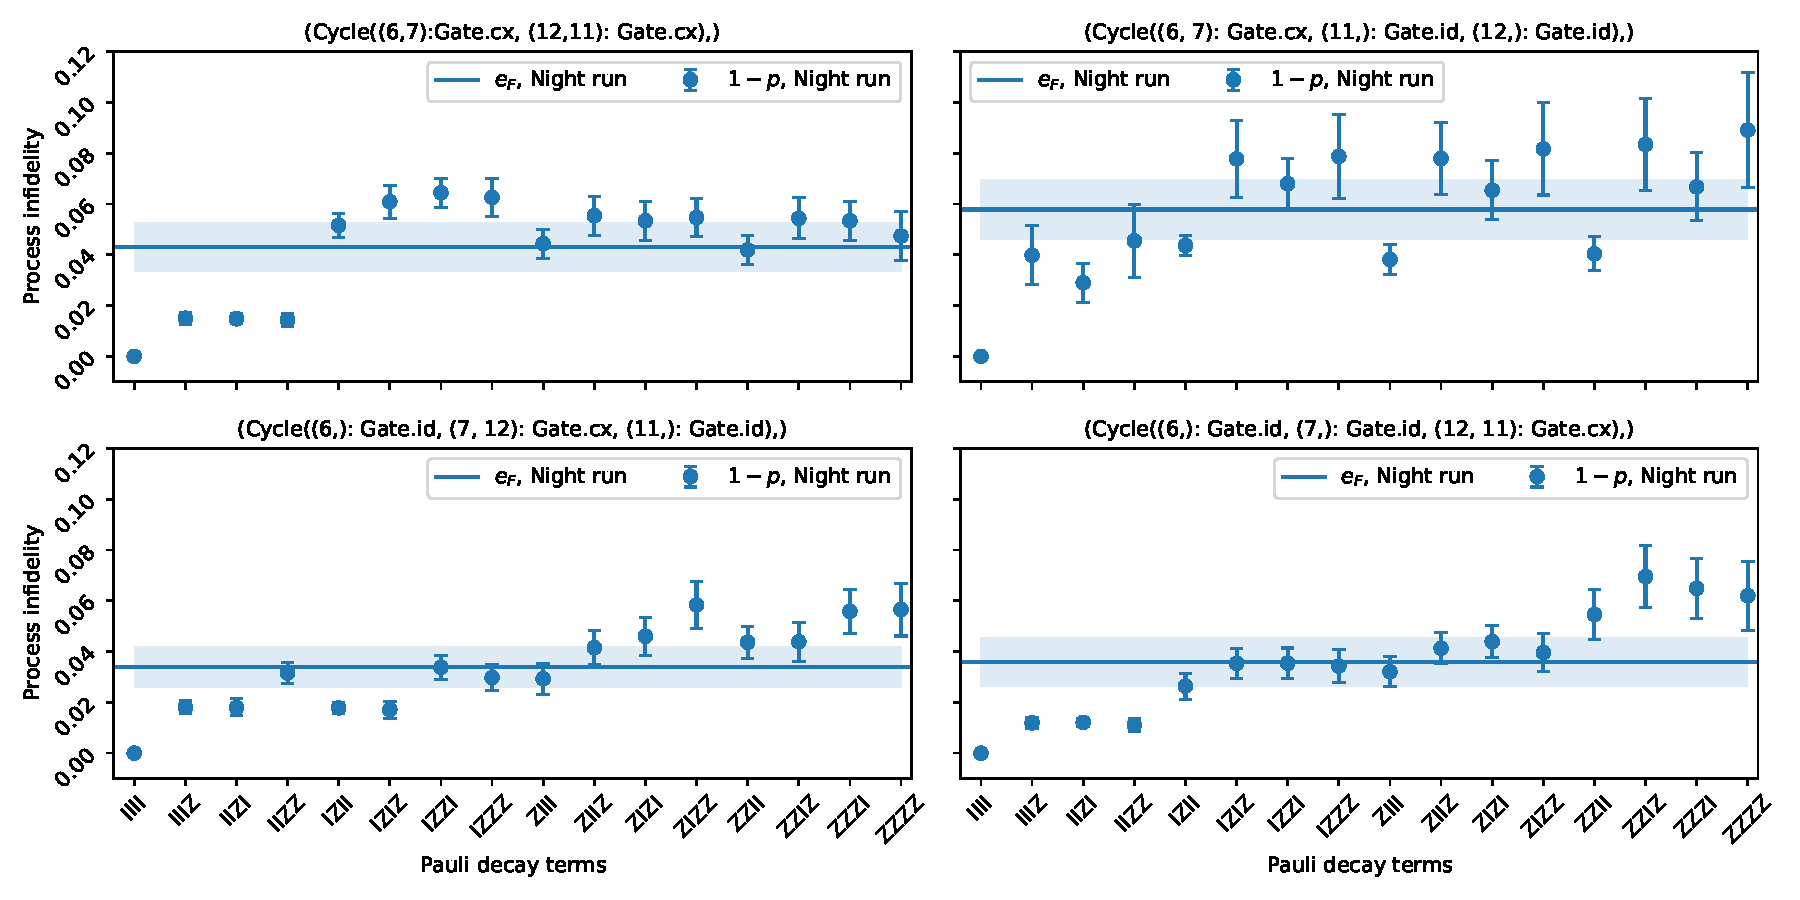
\includegraphics[scale=0.56]{CBPauliInfidelities_27_01_2021_NightRun_Layout2_Cycle1_2_3_4.pdf}
    \caption{The Pauli infidelities for each hard cycle calculated for each Pauli decay term from night run of layout 2 (qubits [6, 7, 12, 11]) on day 01/27/2021. The shaded regions show the error on the process infidelity and the error bars on the markers show the statistical errors on Pauli decay terms. }
    \label{fig:PauliInfidelities27Night_Story6}
\end{figure*}
 
 
 

\begin{figure}[ht!]
    % \centering
    % \includegraphics[width=2.2\columnwidth]{final_plot.pdf}
    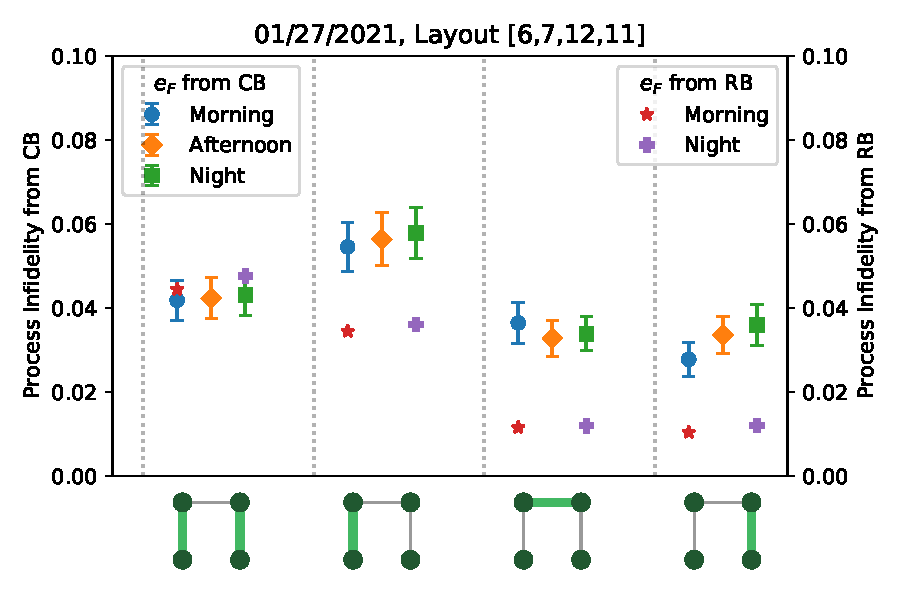
\includegraphics[scale=0.5]{ProcessInfidelities_CB_RB_Data_01_27_2021Layout2aligned.pdf}
    \caption{The process infidelities for cycles  1, 2, 3, and 4 calculated using randomized benchmarking (RB) (right axis) and cycle benchmarking (CB) (left axis) from morning, night, and afternoon runs of layout 2 (qubits [6, 7, 12, 11]) on days 01/27/2021.}
    \label{fig:processinfidelitiesStory6}
\end{figure}

Using this process infidelity information the QCAP bound as a function of number Trotter steps was calculated using cycle benchmarking and compared to the randomized benchmarking data taken from the IBM backend properties for January 27th (Fig.~\ref{fig:QCAPCB_RB_Story6}).

\begin{figure}[ht!]
    % \centering
    % \includegraphics[width=2.2\columnwidth]{final_plot.pdf}
    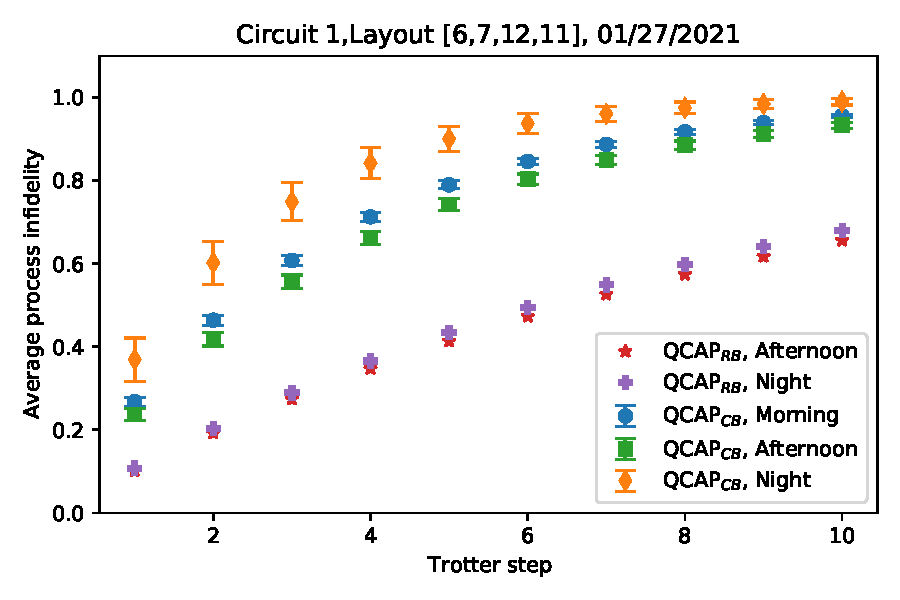
\includegraphics[scale=0.56]{QCAP_CB_RB_Data_01_27_2021_Layout_2C1.pdf}
    \caption{The QCAP bound as a function of number Trotter steps calculated using randomized benchmarking (QCAP$_{\text{RB}}$) (right axis) and cycle benchmarking (QCAP$_{\text{CB}}$) (left axis) from morning and afternoon runs of layout 2 (qubits [6, 7, 12, 11]) on days 01/27/2021.}
    \label{fig:QCAPCB_RB_Story6}
\end{figure}

The particle number in site 1 was calculated from the TIM Hamiltonian computations for the morning, afternoon and evening of January 27th and plotted in Fig.~\ref{fig:n1_Story6}.


\begin{figure}[ht!]
    % \centering
    % \includegraphics[width=2.2\columnwidth]{final_plot.pdf}
    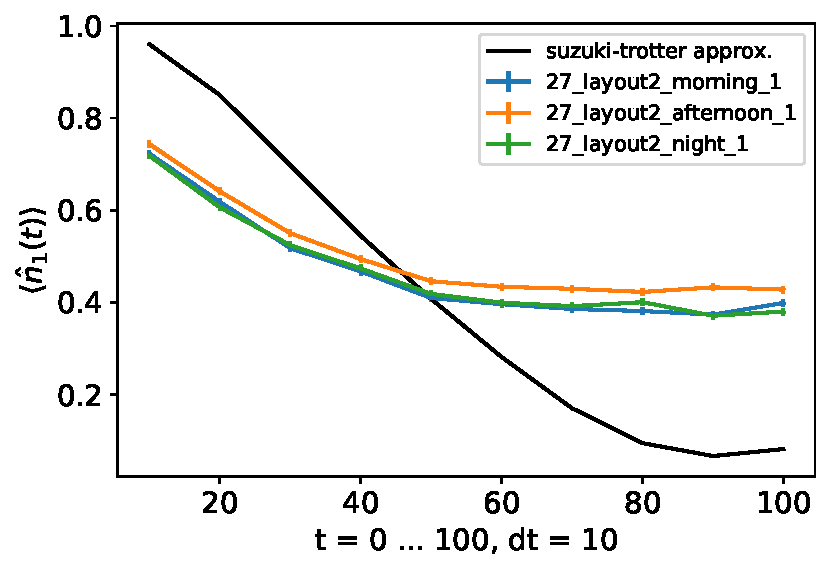
\includegraphics[scale=0.55]{TIM_[27]_[layout2]_[morning, afternoon, night]_n1.pdf}
    \caption{The particle number in site 1 calculated as a function of time from morning, afternoon. and night run of layout 2 (qubits [6, 7, 12, 11]) on days 01/27/2021 compared to exact Suzuki-Trotter approximation.}
    \label{fig:n1_Story6}
\end{figure}

These intra-day calibration drifts occurred regularly each day.  An additional example of this intra-day drift can also be seen from analyzing the detailed variances between the morning and night 2 qubit re-calibrations of qubits 6, 7, 11, and 12 can be also seen in the comparison of the Pauli infidelities for each hard cycle calculated for each Pauli decay term from morning run of layout 2 (qubits [6, 7, 12, 11]) on 01/27/2021 (Figure~\ref{fig:PauliInfidelities30Morning_Story7} and Figure~\ref{fig:PauliInfidelities30Night_Story7} ) 
and the overall process infidelity for cycles 1, 2, 3, and 4 in 
Figure~\ref{fig:processinfidelitiesStory7}



\begin{figure*}[ht!]
    % \centering
    % \includegraphics[width=2.2\columnwidth]{final_plot.pdf}
    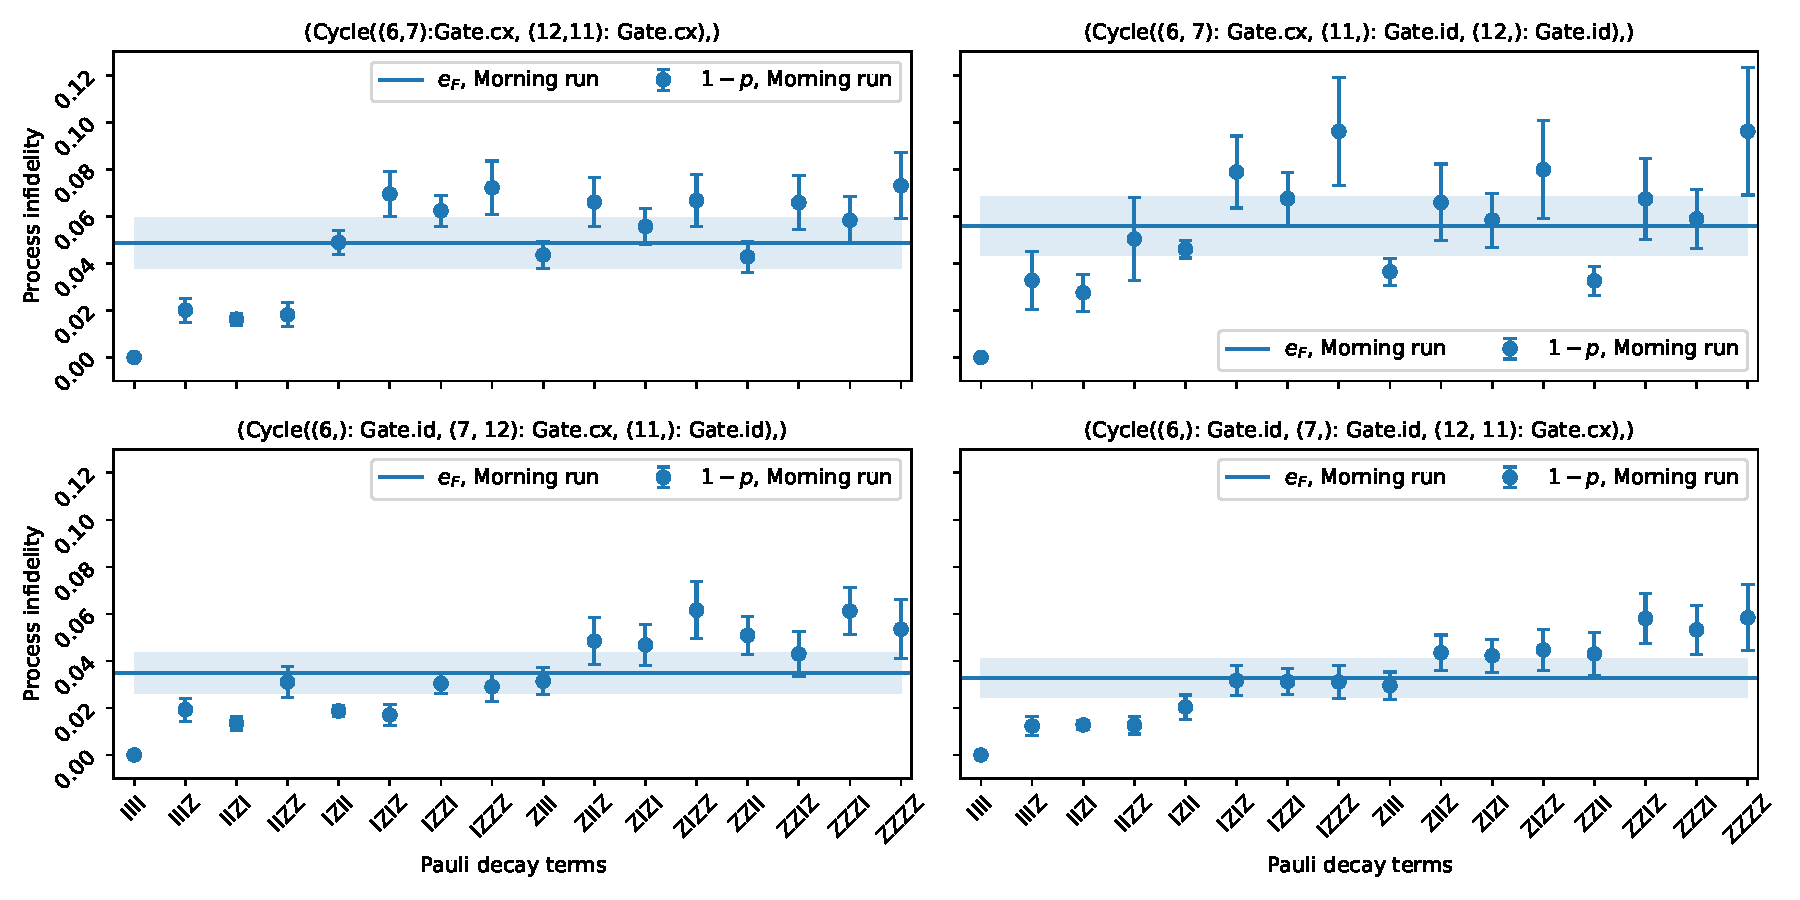
\includegraphics[scale=0.56]{CBPauliInfidelities_30_01_2021_MorningRun_Layout2_Cycle1_2_3_4.pdf}
    \caption{The Pauli infidelities for each hard cycle calculated for each Pauli decay term from morning run of layout 2 (qubits [6, 7, 12, 11]) on day 01/30/2021. The shaded regions show the error on the process infidelity and the error bars on the markers show the statistical errors on Pauli decay terms. }
    \label{fig:PauliInfidelities30Morning_Story7}
\end{figure*}

%\begin{figure*}[ht!]
    % \centering
    % \includegraphics[width=2.2\columnwidth]{final_plot.pdf}
%    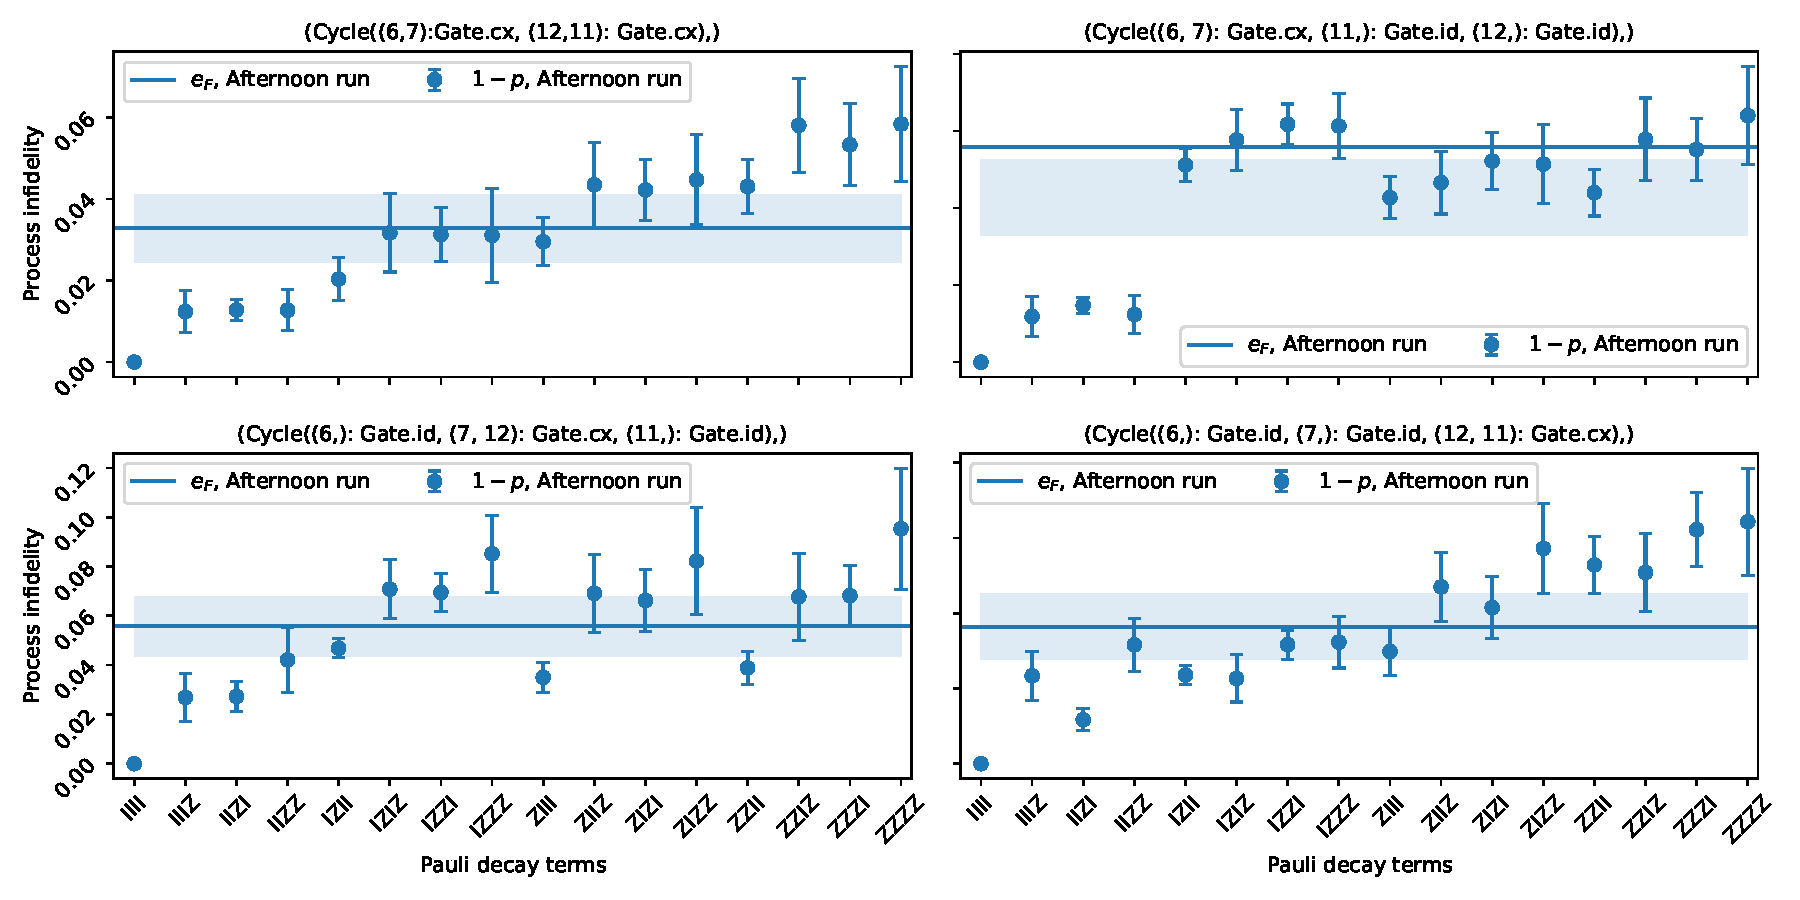
\includegraphics[scale=0.56]{CBPauliInfidelities_30_01_2021_AfternoonRun_Layout2_Cycle1_2_3_4.pdf}
%    \caption{The Pauli infidelities for each hard cycle calculated for each Pauli decay term from afternoon run of layout 2 (qubits [6, 7, 12, 11]) on day 01/30/2021. The shaded regions show the error on the process infidelity and the error bars on the markers show the statistical errors on Pauli decay terms. }
%    \label{fig:PauliInfidelities30Afternoon_Story7}
%\end{figure*}

\begin{figure*}[ht!]
    % \centering
    % \includegraphics[width=2.2\columnwidth]{final_plot.pdf}
    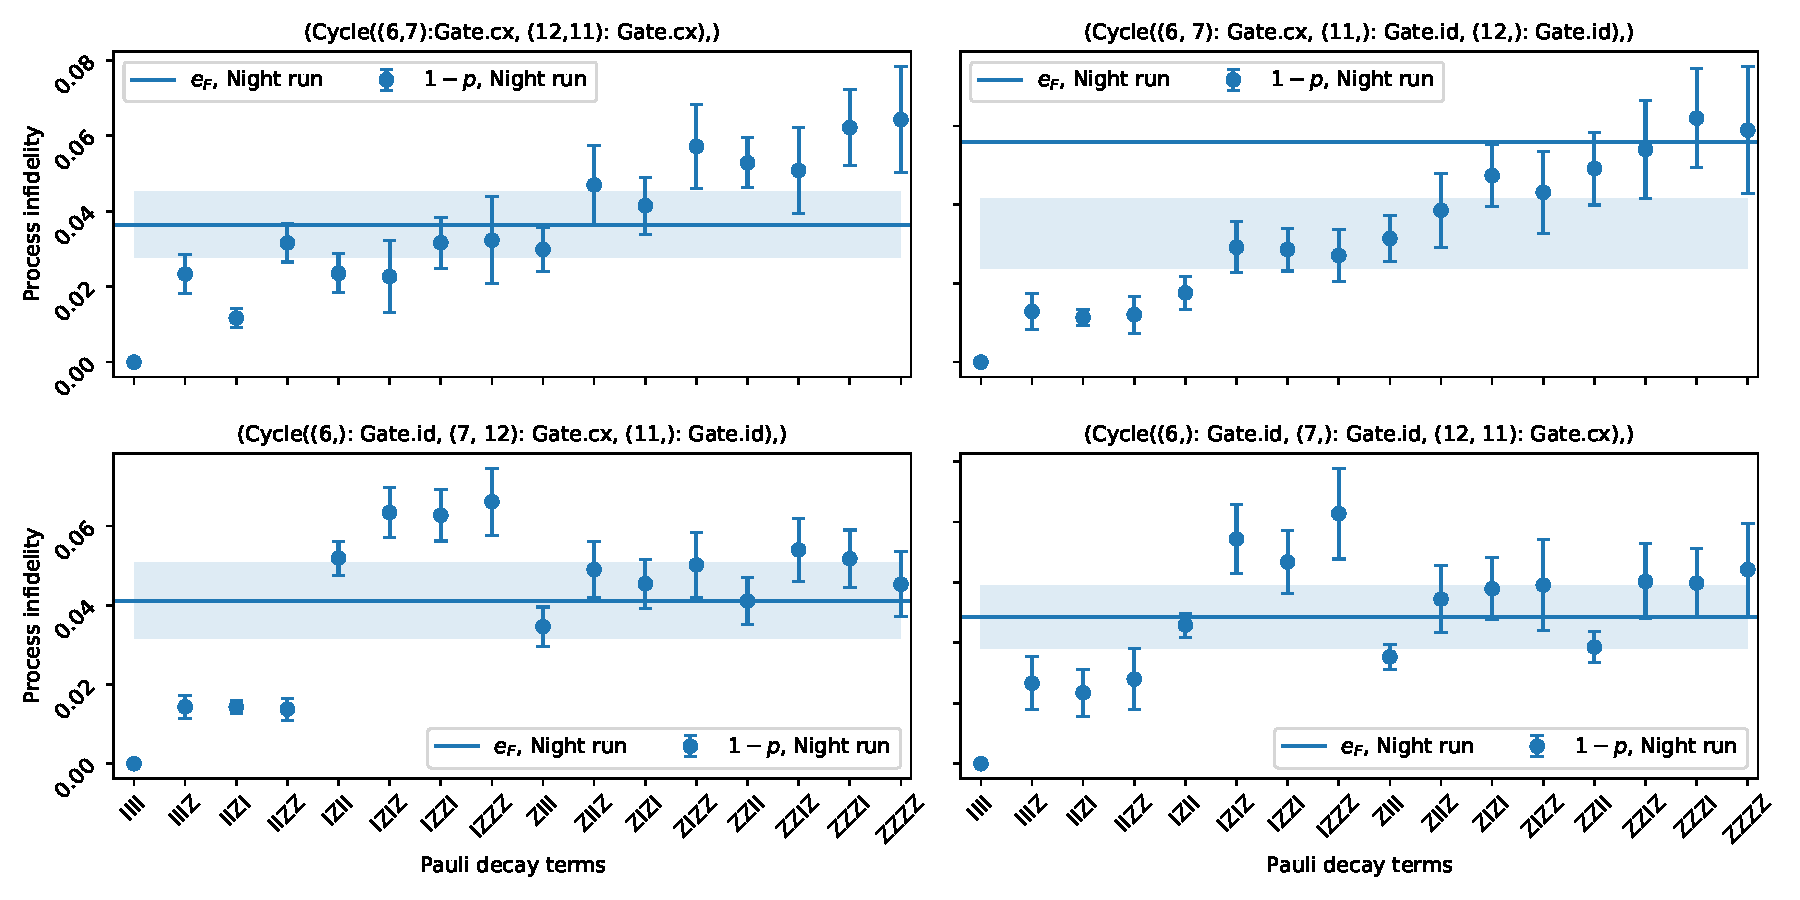
\includegraphics[scale=0.56]{CBPauliInfidelities_30_01_2021_NightRun_Layout2_Cycle1_2_3_4.pdf}
    \caption{ \textbf{NIGHT RUN OF LAYOUT 2} (qubits [6, 7, 12, 11]) on day 01/30/202  The Pauli infidelities for each hard cycle calculated for each Pauli decay term from night run of layout 2 (qubits [6, 7, 12, 11]) on day 01/30/2021. The shaded regions show the error on the process infidelity and the error bars on the markers show the statistical errors on Pauli decay terms. }
    \label{fig:PauliInfidelities30Night_Story7}
\end{figure*}





















\begin{figure}[ht!]
    % \centering
    % \includegraphics[width=2.2\columnwidth]{final_plot.pdf}
    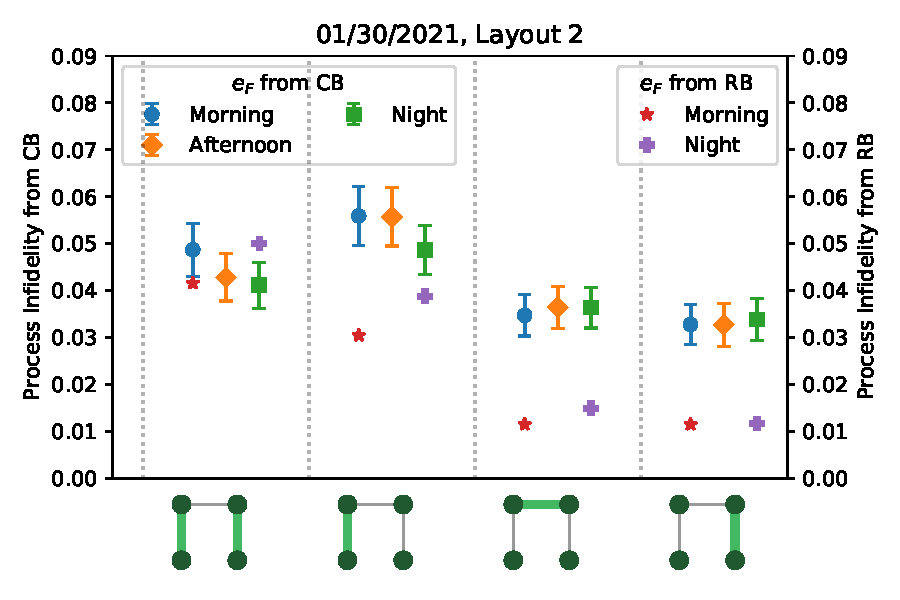
\includegraphics[scale=0.5]{ProcessInfidelities_CB_RB_Data_01_30_2021Layout2aligned.pdf}
    \caption{The process infidelities for cycles  1, 2, 3, and 4 calculated using randomized benchmarking (RB) (right axis) and cycle benchmarking (CB) (left axis) from morning, night, and afternoon runs of layout 2 (qubits [6, 7, 12, 11]) on days 01/30/2021.}
    \label{fig:processinfidelitiesStory7}
\end{figure}


\begin{figure}[ht!]
    % \centering
    % \includegraphics[width=2.2\columnwidth]{final_plot.pdf}
    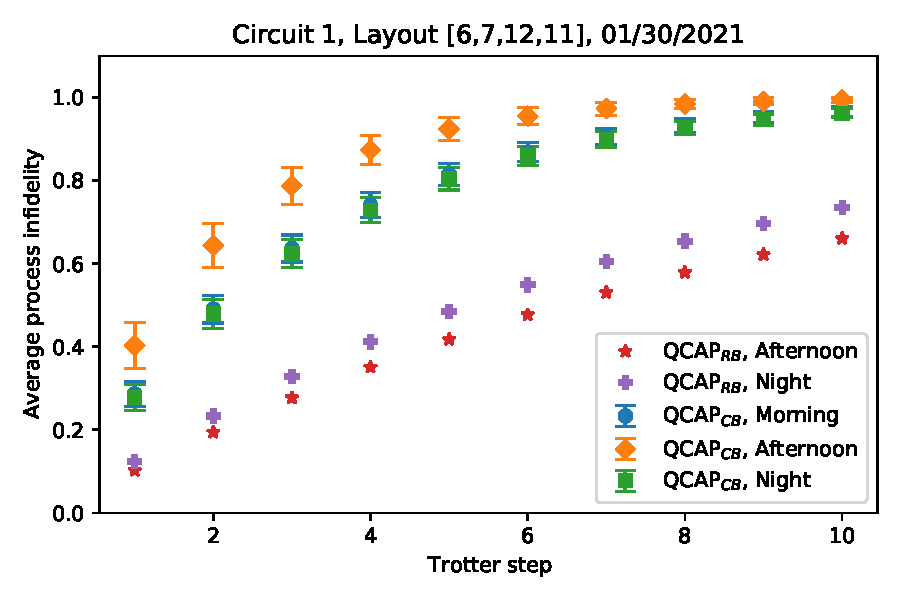
\includegraphics[scale=0.56]{QCAP_CB_RB_Data_01_30_2021_Layout_2C1.pdf}
    \caption{The QCAP bound as a function of number Trotter steps calculated using randomized benchmarking (QCAP$_{\text{RB}}$) (right axis) and cycle benchmarking (QCAP$_{\text{CB}}$) (left axis) from morning and afternoon runs of layout 2 (qubits [6, 7, 12, 11]) on days 01/30/2021.}
    \label{fig:QCAPCB_RB_Story7}
\end{figure}

\begin{figure}[ht!]
    % \centering
    % \includegraphics[width=2.2\columnwidth]{final_plot.pdf}
    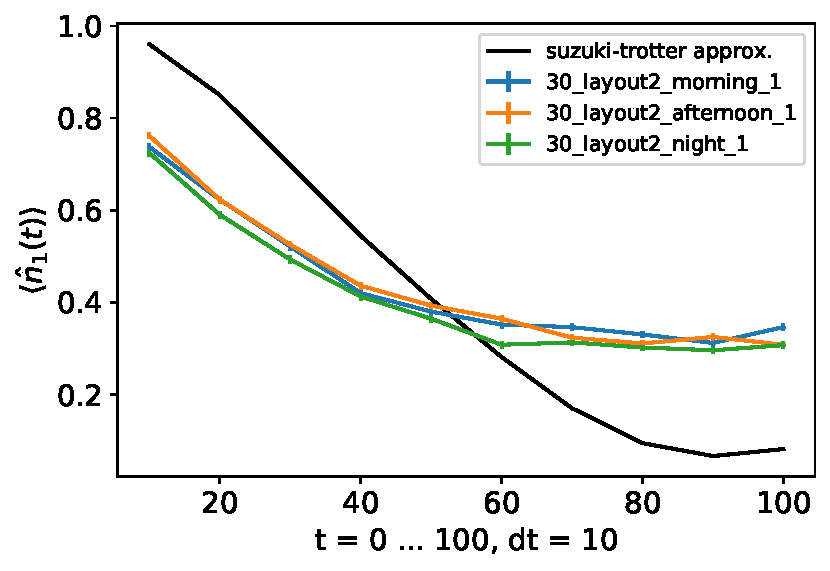
\includegraphics[scale=0.55]{TIM_[30]_[layout2]_[morning, afternoon, night]_n1.pdf}
    \caption{The particle number in site 1 calculated as a function of time from morning, afternoon and night runs on layout 2 (qubits [6, 7, 12, 11]) on day 01/30/2021 compared to exact Suzuki-Trotter approximation.}
    \label{fig:n1_Story7}
\end{figure}



\subsection{Concurrent Computation Inconsistency Using Different QC Hardware Platform Qubits}
\label{sec:concurrent-computation-inconsistency-analysis}


Some researchers have recently put forward the idea of making duplicate copies of their quantum circuit and physically locating them on qubits in different areas of the processor for larger size IBM hardware platforms.  This technique in effect tries to parallelize the computation so that additional data and better statistics for the quantum circuit can be obtained more rapidly.

Our group ran experiments with this technique using cycle benchmarking and selecting a specific date and time to load identical copies of circuit 1 onto qubits located in different physical areas of the hardware platform.  The objective of these measurements was to indeed verify that the quantum hardware platform indeed produced a consistent set of results when comparing the outputs of circuit 1 on these two physically separated set of qubits.

In this section we report on the results of this technique.  We selected circuit 1 for the cycle benchmarking computations and ran this circuit on layout 1 and layout 2 after the IBM night calibration of Boeblingen on January 25th and again after the morning calibrations on January 27th. Figure~\ref{fig:QCAP_CB_RB_Data_01_25_2021_Layout_1_2C1_Night} shows both a graph of the cycle benchmarking average process infidelity versus Trotter step for circuit 1 run on both Layout 1 and 2 and a graph of the measurements from the random benchmarking calibration of Boeblingen by the IBM team after the night calibration on January 25th.  Figure~\ref{fig:QCAP_CB_RB_Data_01_27_2021_Layout_1_2C1_Morning} shows a similar plot for circuit 1 implemented on layout 1 and 2 and a graph of the measurements from the random benchmarking calibration of Boeblingen by the IBM team after the night calibration on January 27th.

What is clear from both graphs is that identical copies of circuit 1 executed on the Boeblingen processor on the same date and time but implemented on different groups of qubits physically separated on the processor produced sufficiently different values of the expected answers that they were beyond any overlap of the error bars of each of the calculations.  Essentially these graphs are indicating that the results from the same calculation implemented in parallel on different physically displaced sets of qubits have only a limited capability to deliver consistent results.



\begin{figure}[H]
    % \centering
    % \includegraphics[width=2.2\columnwidth]{final_plot.pdf}
    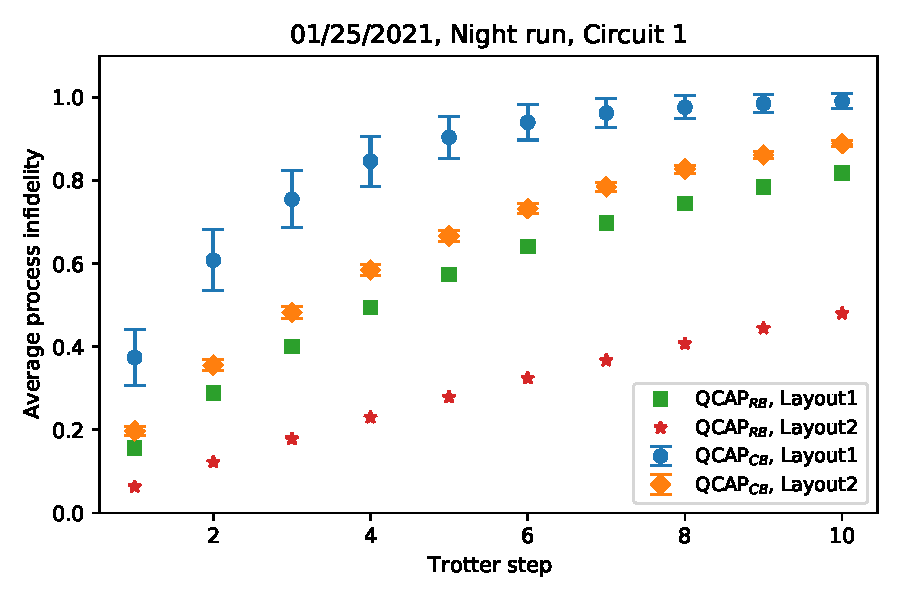
\includegraphics[scale=0.56]{QCAP_CB_RB_Data_01_25_2021_Layout_1_2C1_Night.pdf}
    \caption{The QCAP bound as a function of number Trotter steps calculated using randomized benchmarking (QCAP$_{\text{RB}}$) (right axis) and cycle benchmarking (QCAP$_{\text{CB}}$) (left axis) from the night run of circuit 1 on both layout 1 (qubits [0, 1, 2, 3]) and layout 2 (qubits [6, 7, 12, 11]) on January 25, 2021.}
    \label{fig:QCAP_CB_RB_Data_01_25_2021_Layout_1_2C1_Night}
\end{figure}


\begin{figure}[H]
    % \centering
    % \includegraphics[width=2.2\columnwidth]{final_plot.pdf}
    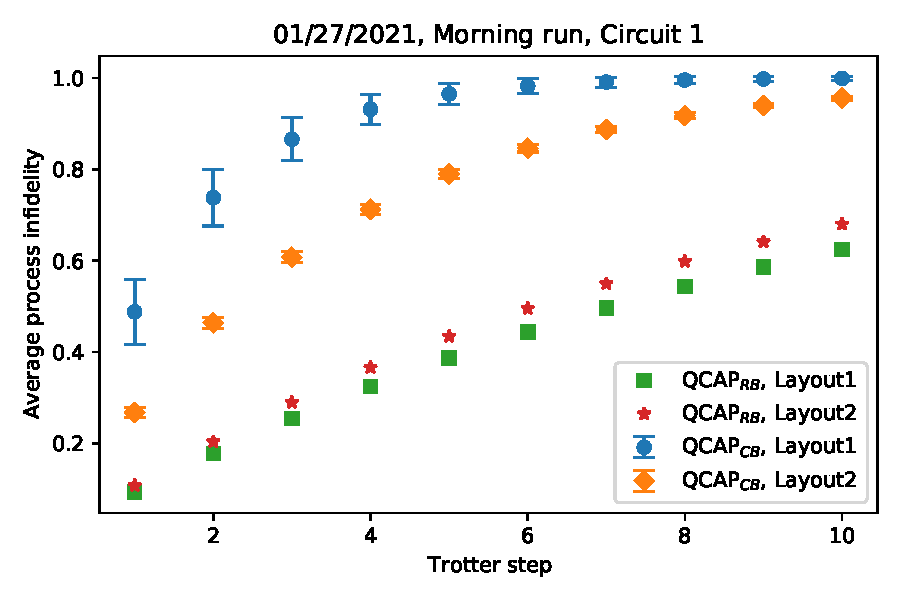
\includegraphics[scale=0.56]{QCAP_CB_RB_Data_01_27_2021_Layout_1_2C1_Morning.pdf}
    \caption{The QCAP bound as a function of number Trotter steps calculated using randomized benchmarking (QCAP$_{\text{RB}}$) (right axis) and cycle benchmarking (QCAP$_{\text{CB}}$) (left axis) from the morning run of circuit 1 on both layout 1 (qubits [0, 1, 2, 3]) and layout 2 (qubits [6, 7, 12, 11]) on January 27, 2021.}
    \label{fig:QCAP_CB_RB_Data_01_27_2021_Layout_1_2C1_Morning}
\end{figure}
















The process infidelity of each cycle obtained using cycle benchmarking and randomized benchmarking for night run on Layout 2 (qubits [6, 7, 12, 11]) on day 01/25/2021 can be seen in Fig.~\ref{fig:processinfidelitiesStory5}.

\begin{figure}[H]
    % \centering
    % \includegraphics[width=2.2\columnwidth]{final_plot.pdf}
    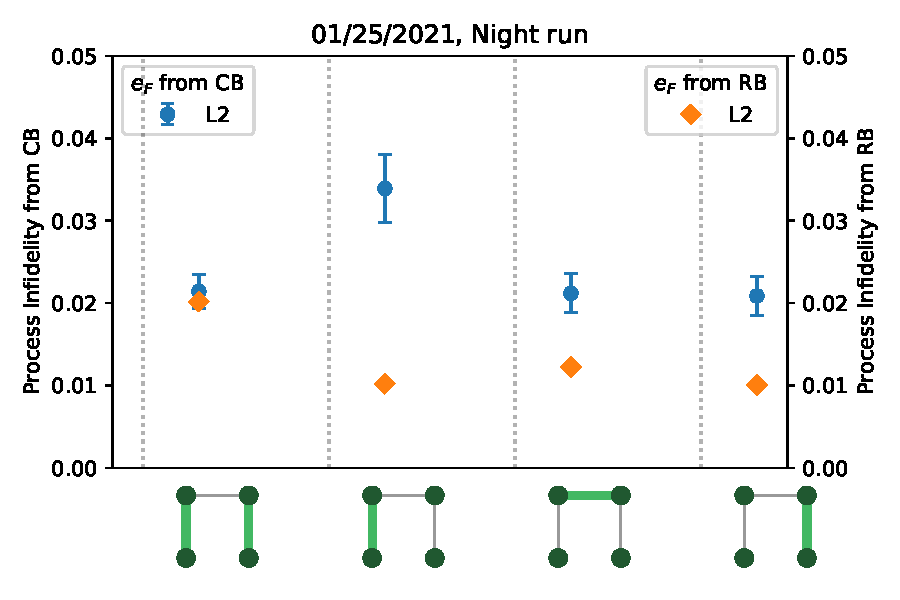
\includegraphics[scale=0.5]{ProcessInfidelities_CB_RB_Data_01_25_2021Layout2aligned.pdf}
    \caption{The process infidelities for cycles  1, 2, 3, and 4 calculated using randomized benchmarking (RB) (right axis) and cycle benchmarking (CB) (left axis) from night run of layout 2 (qubits [6, 7, 12, 11]) on day 01/25/2021.}
    \label{fig:processinfidelitiesStory5}
\end{figure}

The QCAP$_{\text{CB}}$ and QCAP$_{\text{RB}}$ values as a function of number Trotter steps for night run on layout 2 (qubits [6, 7, 12, 11]) on day 01/25/2021 can be seen in Fig.~\ref{fig:QCAPCB_RB_Story5}.

\begin{figure}[H]
    % \centering
    % \includegraphics[width=2.2\columnwidth]{final_plot.pdf}
    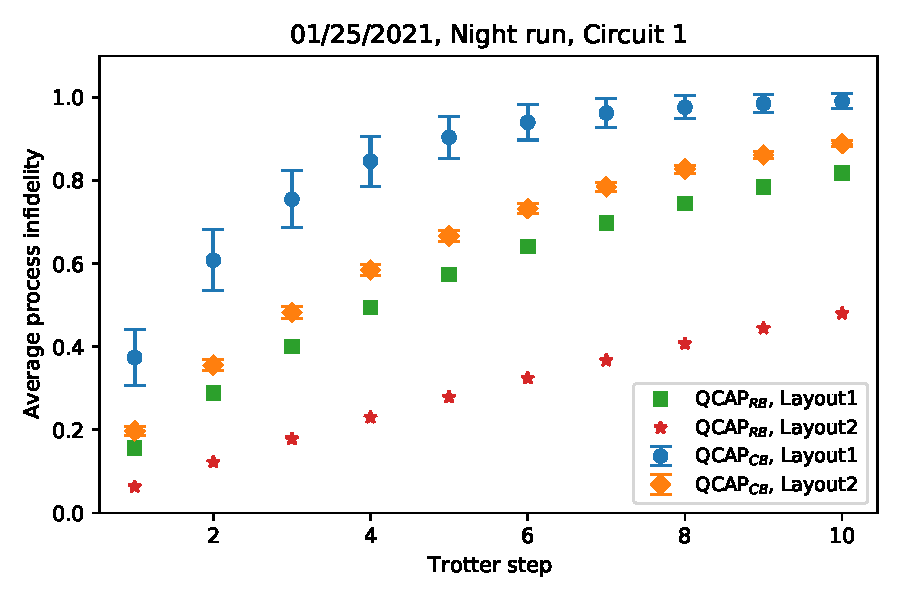
\includegraphics[scale=0.56]{QCAP_CB_RB_Data_01_25_2021_Layout_1_2C1_Night.pdf}
    \caption{The QCAP bound as a function of number Trotter steps calculated using randomized benchmarking (QCAP$_{\text{RB}}$) (right axis) and cycle benchmarking (QCAP$_{\text{CB}}$) (left axis) from night run of layout 2 (qubits [6, 7, 12, 11]) on day 01/25/2021.}
    \label{fig:QCAPCB_RB_Story5}
\end{figure}

The particle number in site 1 as a function of time comparing exact Trotter values with the values obtained from night run on layout 1 (qubits [0,1,2,3]) and 2 (qubits [6, 7, 12, 11]) on day 01/25/2021 can be seen in Fig.~\ref{fig:n1_Story5}.

\begin{figure}[H]
    % \centering
    % \includegraphics[width=2.2\columnwidth]{final_plot.pdf}
    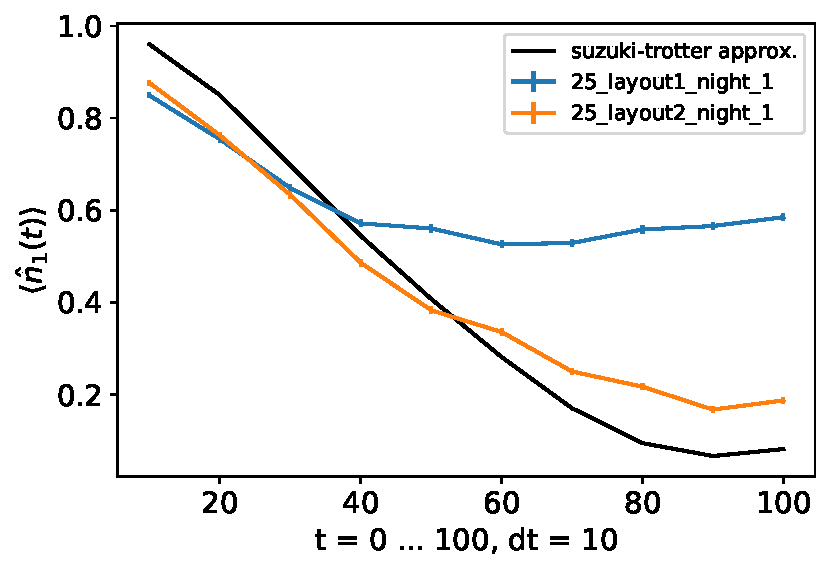
\includegraphics[scale=0.55]{TIM_[25]_[layout1, layout2]_[night]_n1.pdf}
    \caption{The particle number in site 1 calculated as a function of time from night run on layout 1 (qubits [0, 1, 2, 3]) and layout 2 (qubits [6, 7, 12, 11]) on day 01/25/2021 compared to exact Suzuki-Trotter approximation.}
    \label{fig:n1_Story5}
\end{figure}

\begin{figure*}[H]
    % \centering
    % \includegraphics[width=2.2\columnwidth]{final_plot.pdf}
    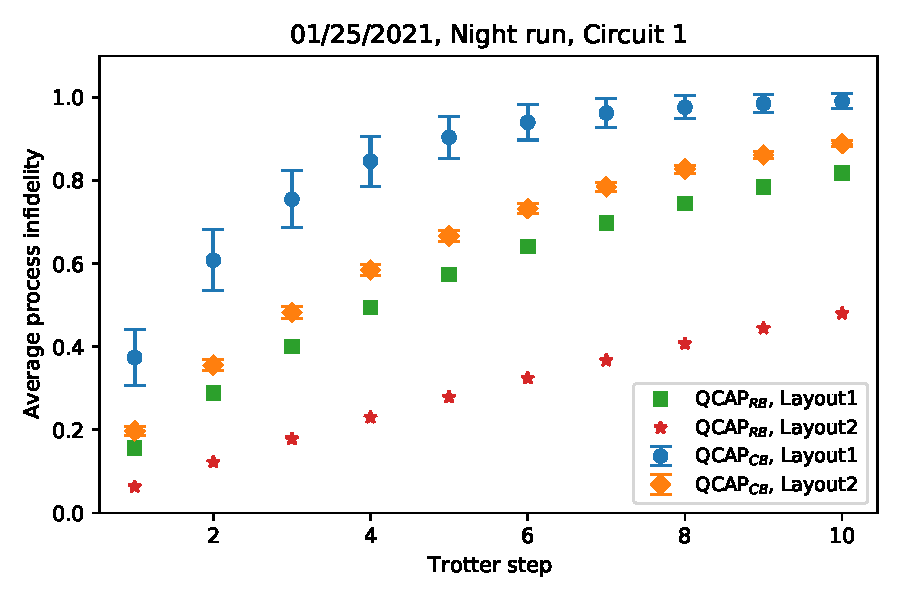
\includegraphics[scale=0.55]{QCAP_CB_RB_Data_01_25_2021_Layout_1_2C1_Night.pdf}
    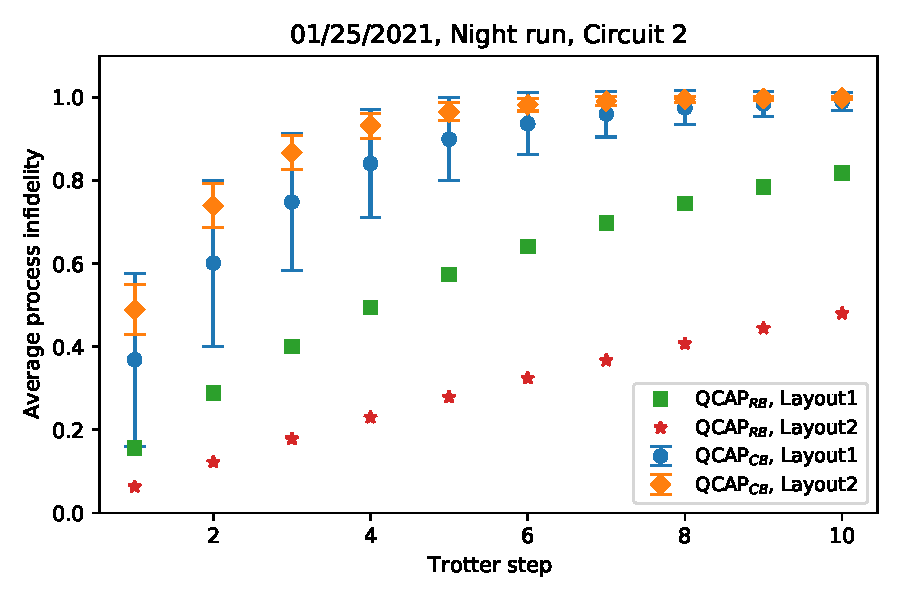
\includegraphics[scale=0.55]{QCAP_CB_RB_Data_01_25_2021_Layout_1_2C2_Night.pdf}
    \caption{The QCAP bound as a function of number Trotter steps calculated using randomized benchmarking (QCAP$_{\text{RB}}$) and cycle  benchmarking (QCAP$_{\text{CB}}$) from night run of layout 1 and 2 on day 01/25/2021 for Circuit 1 (left panel) and Circuit 2 (right panel) with only CNOT gates used as hard cycles. The  plotted  error  bars  only show the statistical error.}
    \label{fig:QCAP_circ1_circ2_25th_L1L2_Night}
\end{figure*}





\subsection{QCAP Bound Performance of Different Gate Combination Giving the Same Physics}
\label{sec:circ1_vs_circ2_QCAP}

In this section, we discuss the QCAP bound performance of the two quantum circuits as seen in Fig.~\ref{fig:IsingTrotterCircs} with different gate layout for TIM Trotter step that gives the same physics. As discussed above, in our QCAP calculations we used CNOT gates as our hard gates since two-qubit errors are the dominant source of error in the quantum circuit. Therefore, we can say that the QCAP bound values that we calculated are lower bound to the exact error due to errors in single and two-qubit gates in the quantum circuit. The hard cycles used at each Trotter step for circuit 1 and circuit 2 can be seen in Fig.~\ref{fig:hardcycles}.  
\begin{figure}[ht!]
    % \centering
    % \includegraphics[width=2.2\columnwidth]{final_plot.pdf}
    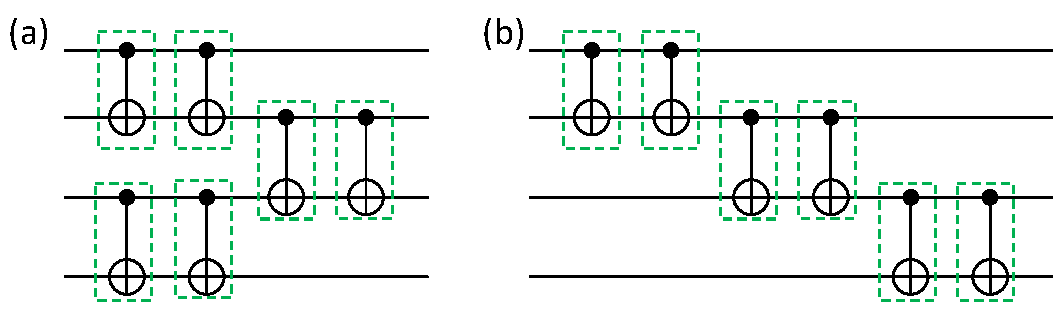
\includegraphics[scale=0.50]{hardcyclesCirc1Circ2.pdf}
    \caption{The CNOT hard cycles used at each Trotter step for circuit 1 ({\bf{(a)}}) and circuit 2 ({\bf{(b)}}) to calculate QCAP$_{\text{CB}}$ bound from cycle benchmarking are shown in dashed boxes.}
    \label{fig:hardcycles}
\end{figure}
% \begin{figure*}[ht!]
%     % \centering
%     % \includegraphics[width=2.2\columnwidth]{final_plot.pdf}
%     \includegraphics[scale=0.55]{QCAP_CB_RB_Data_01_24_2021_Layout_2C1_C2_Morning.pdf}
%     \includegraphics[scale=0.55]{QCAP_CB_RB_Data_01_29_2021_Layout_2C1_C2_Morning.pdf}
%     \caption{The QCAP bound as a function of number Trotter steps calculated using randomized benchmarking (QCAP$_{\text{RB}}$) and cycle  benchmarking (QCAP$_{\text{CB}}$) from morning run of layout 2 (qubits [6, 7, 12, 11]) on days 01/24/2021 (left panel) and 01/29/2021 (right panel) for Circuit 1 and Circuit 2 with only CNOT gates used as hard cycles. The  plotted  error  bars  only show the statistical error.}
%     \label{fig:QCAP_circ1_circ2_24th_29th_L2_Morning}
% \end{figure*}

% \begin{figure}[ht!]
%     % \centering
%     \includegraphics[scale=0.55]{QCAP_CB_RB_Data_01_25_2021_Layout_2C1_C2_Morning.pdf}
%     \caption{The QCAP bound as a function of number Trotter steps calculated using randomized benchmarking (QCAP$_{\text{RB}}$) and cycle  benchmarking (QCAP$_{\text{CB}}$) from morning run of layout 2 on day 01/25/2021 for Circuit 1 and Circuit 2 with only CNOT gates used as hard cycles. The  plotted  error  bars  only show the statistical error.}
%     \label{fig:QCAP_circ1_circ2_25th_L2_Morning}
% \end{figure}

\begin{figure*}[ht!]
    % \centering
    % \includegraphics[width=2.2\columnwidth]{final_plot.pdf}
    \includegraphics[scale=0.36]{QCAP_CB_RB_Data_01_24_2021_Layout_2C1_C2_Morning.pdf}
    \includegraphics[scale=0.36]{QCAP_CB_RB_Data_01_25_2021_Layout_2C1_C2_Morning.pdf}
    \includegraphics[scale=0.36]{QCAP_CB_RB_Data_01_29_2021_Layout_2C1_C2_Morning.pdf}
    \caption{The QCAP bound as a function of number Trotter steps calculated using randomized benchmarking (QCAP$_{\text{RB}}$) and cycle  benchmarking (QCAP$_{\text{CB}}$) from morning run of layout 2 (qubits [6, 7, 12, 11]) on days 01/24/2021 (left panel), 01/25/2021 (middle panel) and 01/29/2021 (right panel) for Circuit 1 and Circuit 2 with only CNOT gates used as hard cycles. The  plotted  error  bars  only show the statistical error.}
    \label{fig:QCAP_circ1_circ2_24th_25th_29th_L2_Morning}
\end{figure*}
In Fig.~\ref{fig:QCAP_circ1_circ2_24th_25th_29th_L2_Morning} we demonstrate the QCAP$_{\text{CB}}$ bound for the CNOT hard cycles in circuit 1 and circuit 2 (Fig.~\ref{fig:hardcycles}) as a function of Trotter steps for morning run on layout 2 (qubits [6,7,11,12]) on days 01/24-25-29/2021, respectively. These figures show that the QCAP$_{\text{CB}}$ bound for circuit 2 is higher than the QCAP$_{\text{CB}}$ bound for circuit 1. This is an expected result as the quantum circuit depth for circuit 2 is greater than the circuit depth for circuit 1. However, these results are interesting since they show how fast the QCAP$_{\text{CB}}$ bound can grow when the order of gates is not done wisely. On the other hand, since individual CNOT gates are used when the process infidelity is calculated from randomized benchmarking the QCAP$_{\text{RB}}$ bound calculated from \eqref{eq:QCAP_RB} does not depend on the CNOT layout in the circuit, i.e. it only depends on the number of CNOT gates in the circuit. Therefore, it does not reflect how fast the errors can grow in the quantum circuit depending on the circuit depth.